\documentclass[12pt]{article}

\usepackage{graphicx}
\usepackage{amsmath}
\usepackage{amssymb}
\usepackage{natbib}
\usepackage{amsfonts}
\usepackage{multicol}
\usepackage{float}
\usepackage{oldgerm}
\usepackage{bm}
\usepackage{mathtools}
\usepackage{wrapfig}
\usepackage{fancyhdr}
\usepackage[export]{adjustbox}
\usepackage{xcolor}

\pagestyle{empty}

\newcommand{\avec}{{\mathbf A}}
\newcommand{\bvec}{\mathbf B}
\newcommand{\dvec}{\mathbf D}
\newcommand{\evec}{\mathbf E}
\newcommand{\fvec}{\mathbf F}
\newcommand{\jvec}{\mathbf J}
\newcommand{\kvec}{{\mathbf {k}}}
\newcommand{\mvec}{{\mathbf {M}}}
\newcommand{\nbold}{{\mathbf n}}
\newcommand{\vvec}{\mathbf{v}}
\newcommand{\xvec}{{\mathbf x}}
\newcommand{\yvec}{{\mathbf y}}
\newcommand{\zvec}{{\mathbf z}}
\newcommand{\nablav}{\boldsymbol{\nabla}}
\newcommand{\phivec}{\boldsymbol{\phi}}
\newcommand{\epvec}{\boldsymbol{\epsilon}}
\newcommand{\ezero}{\epsilon_{0}}
\newcommand{\mzero}{\mu_{0}}
\newcommand{\unitx}{\mathbf{\hat{x}}}
\newcommand{\unity}{\mathbf{\hat{y}}}
\newcommand{\unitz}{\mathbf{\hat{z}}}
\newcommand{\mubold}{\boldsymbol{\mu}}
\newcommand{\uniti}{\hat{\boldsymbol{\imath}}}
\newcommand{\unitj}{\hat{\boldsymbol{\jmath}}}
\newcommand{\unitk}{\hat{\boldsymbol{\mathit{k}}}}
\newcommand{\unitn}{\hat{\mathbf n}}
\newcommand{\unitr}{\hat{\mathbf r}}
\newcommand{\unitphi}{\hat{\boldsymbol{\phi}}}
\newcommand{\unittheta}{\hat{\boldsymbol{\theta}}}

\newcommand{\bit}{\begin{itemize}}
\newcommand{\eit}{\end{itemize}}

\setlength{\headsep}{0.5cm}
\setlength{\oddsidemargin}{-0.5cm}
\setlength{\textwidth}{16.5cm}
\setlength{\textheight}{24cm}
\voffset = -2cm

\pagestyle{fancy}
\fancyhf{}
\rfoot{\includegraphics[width=1.0in]{cnm.png}}
\lfoot{Homework 1}
\begin{document}

%{\bf \underline{STUDENT NAME}:} 
%\vspace{1cm}

\begin{center}
%\date{10/02/18-10/09/18}
\hfil
{\large\bf {ENGR 2910-101: Circuit Analysis}}
\hfill Instructor: Brian Rashap\\
Homework 1: 01/11/23 \hfill Due: 01/18/23\\
\hrulefill\\
\end{center}

%{\em Show all your working to ensure you obtain full points. Partial
%  credit will be given for correct algebraic steps if you fail to
%  obtain the correct final answer.}\\

%\newpage


\noindent
{\bf Question 1} [10] %P1.12

When a car has a dead battery, it can often be started by connecting
the battery from another car across its terminals. The positive
terminals are connected together as are the negative terminals. The
connection is illustrated in the figure below. Assume the current $i$
in the Figure is measured and found to be 40 A.
\begin{figure}[h!]
  \centering 
  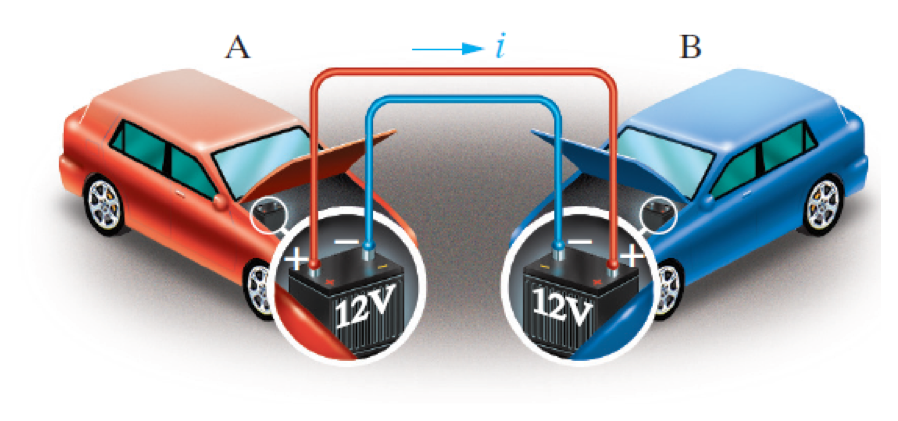
\includegraphics[clip,width=0.5\textwidth]{Fig1-12.eps}
\end{figure}
\bit

\item[(a)]

  Which car has the dead battery?

\item[(b)]

  If this connection is maintained for 90 seconds, how much energy is
  transferred to the dead battery?

\eit

\vspace{0.1in}
\noindent
{\bf Question 2} [10] %P1.13

Two electric circuits, represented by boxes A and B, are connected as
shown in the figure below. The reference direction for the current $i$
in the interconnection and the reference polarity for the voltage $v$
across each interconnect are shown. For each of the following sets of
values, calculate the power in the interconnection and state whether
the power is flowing from A to B or vice versa. 
\begin{figure}[h!]
     \centering
     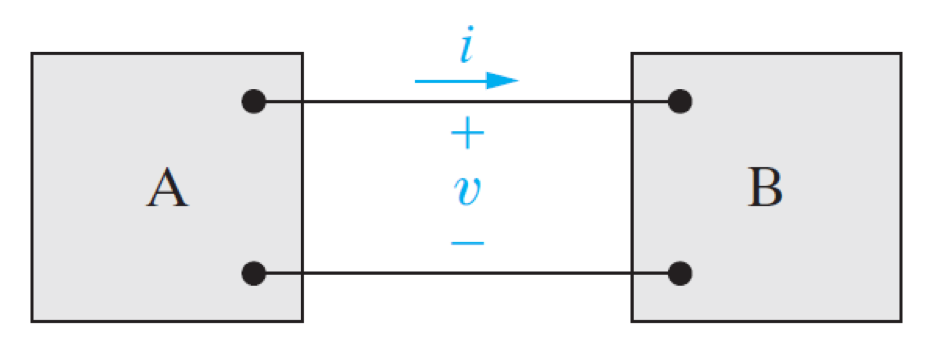
\includegraphics[clip,width=0.3\textwidth]{Fig1-13.eps}
\end{figure}
 \bit

\item[(a)]
$i = 6$ A, $v = 30$ V 

\item[(b)]
$i = -8$ A, $v = -20$ V 

\item[(c)]
$i = 4$ A, $v = -60$ V 

\item[(d)]
$i = -9$ A, $v = 40$ V 

\eit

\vspace{0.1in}
\noindent
{\bf Question 3} [10] %P1-23

The voltage and current at the terminals of the circuit shown below
are zero for $t < 0$ and $t > 40$s. In the interval between 0 s and 40
s, 
\[
v(t) = t( 1 - 0.025 t )~\text{V}~,~ 0 < t < 40 \text{ s}; 
\]
\[
i(t) = 4 - 0.2 t~\text{A}~,~ 0 < t < 40 \text{ s}.
\]
\begin{figure}[h!]
  \centering 
  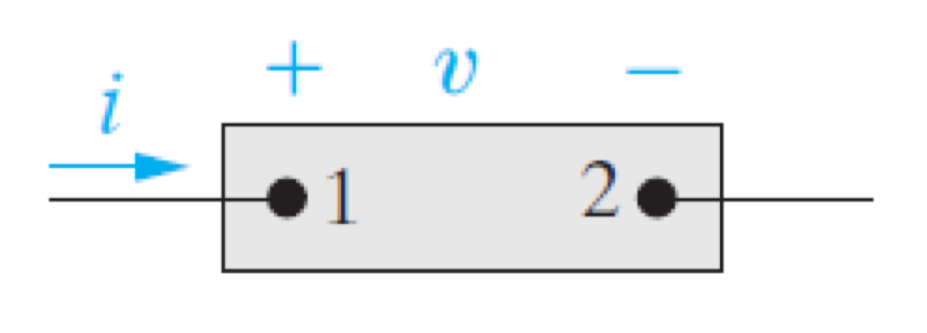
\includegraphics[clip,width=0.25\textwidth]{Fig1-5.eps}
\end{figure}
\bit

\item[(a)]

At what instant of time is the power being delivered to the circuit
element maximum?

\item[(b)]

What is the power at the time found in (a)?

\item[(c)]

  At what instant of time is the power being extracted from the
  circuit maximum?

\item[(d)]

What is the power at the time from (c)?

\item[(e)]

Calculate the net energy delivered to the circuit at 0, 10, 20, 30,
and 40 s.

\eit

\vspace{0.1in}
\noindent 
{\bf Question 4} [10] %P1-20

The voltage and current at the terminals of the above circuit element
are zero for $t<0$. For $t \geq 0$:
\[
v (t) = (1500 t + 1)  e^{-750 t}~\text{V},
\]
\[
i(t) = 40 e^{-750 t}~\text{mA}.
\]
\bit
\item[(a)]

  At what time is the power delivered a maximum?

\item[(b)]

  Find the value of the maximum power in mW.

\item[(c)]

  Find the total energy delivered to the circuit element in $\mu$J.

\eit

\vspace{0.1in}
\noindent
{\bf Question 5} [10] %P2-11

Given the following circuit: 
\begin{figure}[h!]
\centering 
\includegraphics[clip,width=0.35\textwidth]{HW_1_5.png}
\end{figure}
 \bit

\item[(a)]

  Find the current i. 

\item[(b)]

  Find the power supplied by the voltage source.
  
\item[(c)]

  Reverse the polarity of the voltage source and repeat parts (a) and (b).

\eit

\end{document}
